% --- SOCIAL AND ECONOMICAL CONTEXT --- %
\section{Social and economical context}

During the last decades, the amount of unmanned spacecrafts orbiting our planet
has dramatically increased. The main reason behind this situation is the rise of
private launchers and manufacturers, who have lowered the costs, enabling others
to get access to space. This lead to a new aerospace race driven by cheap
technologies, usually referred to as \textit{New Space}, which provide agile,
responsive and simpler solutions to common aerospace tasks.

In addition, a huge demand of communication services is already being experience
by the aerospace market.  Nowadays, this sector generates benefits over $100$
billion euros due to new improvements in satellites' software and hardware, see
\cite{airbus2021}.  Communication services have a variety of purposes, from
in-flight connectivity to network-centric warfare, which are fulfilled by making
use of satellite constellations in order to guarantee a permanent coverage over
particular areas of the globe.

% Reference
% https://www.airbus.com/public-affairs/brussels/our-topics/space/new-space.html

\begin{figure}[h]
  \centering
  \includegraphics[width=\linewidth]{sat_evolution.png}
  \caption[Launched satellites per year.]{Amount of satellites launched during last decades and filtered by their
    mission purpose: space science, Earth observation and communication. This
    last one, shows a big growth rate specially during the last five years. Data
    was obtained and processed from the UCS Satellite Database.}
  \label{fig:sat_evolution}
\end{figure}

All previous satellites' missions, shown in figure \ref{fig:sat_evolution}, are
designed to take place at particular locations of space, as some of those orbits
require specific altitudes and inclinations: geostationary, sun-synchronous...
However, space is a very hostile environment and orbit perturbations exist due
to air drag, Earth's oblateness, third body presence or solar radiation pressure
among many others. These perturbations might originate a shift in the initial
orbit, making it necessary to maneuver the satellite to original desired
position. Orbit corrections require from targeting algorithms which, in the end,
are Lambert's problem solvers.

Within the frame of aerospace sector, a new professional profile is being
demanded by companies: the computer scientist. These people are usually
engineers who have a deep knowledge in both high-performance computing and
mathemtatics modelling the problem. This is one of the reasons behind why many
modern papers, which devise a new approach for the Lambert's problem, include
algorithms in the form of code flowcharts, pseudo-code or links to repositories
hosting original source computer routines.

\begin{figure}[h]
  \centering
  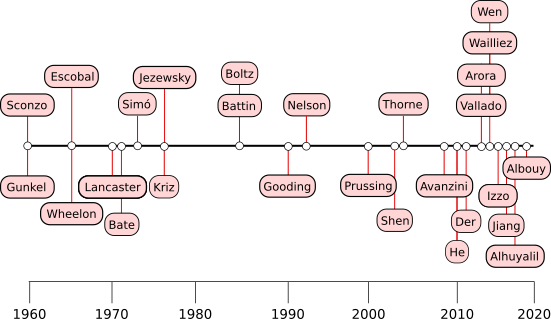
\includegraphics[width=\linewidth]{static/solvers_timeline.png}
  \caption[Publications related with Lamebert's problem.]{More than a dozen of papers have been published over the last twenty
    years. The nature of the proof solutions has evolved also during time, going
    from pure geometric demonstrations to graphic processing units based or even machine
    learning ones.}
  \label{fig:art_lambert}
\end{figure}

